\chapter{Data Mining}
\begin{figure}[ht!]
    \centering
    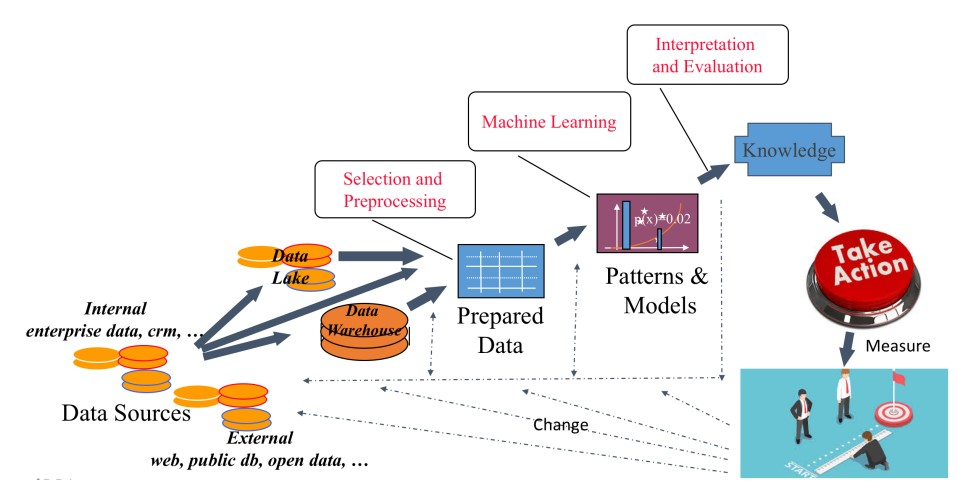
\includegraphics[scale=0.6]{images/Data_Mining_process.jpg}
    \caption{The Data Mining Process}
\end{figure}

\textbf{\textit{Data Mining}} is the process of discovering patterns, trends, correlations, or meaningful information from large datasets. It involves the application of various techniques from \textit{statistics}, \textit{machine learning}, and \textit{database systems} to extract valuable knowledge from raw data.

\section{Business Intelligence and Data Warehouses}

\paragraph{Business Intelligence (BI)}
\textbf{\textit{Business Intelligence (BI)}} represents a key concept in the field of Data Mining and can be described as the process of:
\begin{itemize}
    \item transforming raw data into useful information to support effective and aware business strategies
    \item capturing the business data and getting the right information to the right \textit{people}, at the right \textit{time}, through the right \textit{channel}.
\end{itemize}
There are different definition that has been provided during the years, but there are two of them in particular that we can highlight:
\begin{quote}
    \textit{Business intelligence (BI) is an umbrella term that includes the applications, infrastructure and tools, and best practices that enable access to and analysis of information to improve and optimize decisions and performance. - \textbf{Gartner}}
\end{quote}
\begin{quote}
    \textit{Business Intelligence is a set of methodologies, processes, architectures, and technologies that transform raw data into meaningful and useful information used to enable more effective strategic, tactical, and operational insights and decision-making. - \textbf{Forrester Research}}
\end{quote}

\paragraph{Data Warehouse (DWH)}
One of the main tools to support BI is the \textbf{\textit{Data Warehouse (DWH)}}, which is a type of \textit{Decision Support System (DSS)} and can be seen informally as an optimized repository that stores information for the decision-making process. With the huge and increasing number of information that companies have to manage in order to find relevant business strategies DWHs answer to the necessity of more sophisticated solutions than classical operational databases.\\
The main advantages are the following:
\begin{itemize}
    \item they provide the ability to manage sets of historical data;
    \item they provide the ability to run multidimensional analysis accurately and rapidly;
    \item they are based on a simple model that can be easily learned by its users;
    \item they are the basis for indicator-calculating systems.
\end{itemize}

More formally, we can say that a \textbf{\textit{Data Warehouse (DWH)}} is a specialized database that stores large volumes of historical data and facilitates the analysis and reporting of that data to support \textit{decision-making processes}. It provides several key features:

\begin{itemize}
    \item \textbf{Subject-Oriented:} A data warehouse is designed to focus on specific subjects or domains relevant to the enterprise's operations, such as customers, products, sales, etc. By organizing data around these core concepts, it enables analysts and decision-makers to gain insights into various aspects of the business.

    \item \textbf{Integration and Consistency:} One of the primary functions of a DWH is to integrate data from multiple disparate sources, including transactional databases, spreadsheets, and external systems. This integration ensures that data from different sources is harmonized and provides a unified view across the organization. Consistency in data representation and structure is maintained to ensure accuracy and reliability in analysis.

    \item \textbf{Evolution Over Time and Non-Volatility:} A crucial aspect of a data warehouse is its ability to capture and track changes in data over time. Historical data are preserved, allowing for the analysis of trends and patterns spanning various time periods. Unlike transactional databases where data may be constantly updated or overwritten, data in a data warehouse are non-volatile. Once committed, the data remains static, read-only, and preserved for future reporting and analysis.

\end{itemize}

In summary, a \textbf{\textit{DWH}} serves as a centralized repository for historical data, providing a comprehensive and consistent view of the organization's information assets. By offering subject-oriented, integrated, and non-volatile data, it empowers decision-makers with valuable insights for strategic planning, performance analysis, and informed decision-making.

\paragraph{Data Mart (DM)}
A \textbf{Data Mart (DM)} serves as a specialized subset or aggregation of the data stored within a primary DWH. Unlike the comprehensive nature of a DWH, a \textbf{DM} contains a focused set of information tailored to \textit{meet the needs of a specific business area}, corporate department, or category of users.

One of the key roles of \textbf{DMs} is to act as building blocks during the incremental development of DWHs. Rather than attempting to construct an entire DWH in one go, organizations often adopt an iterative approach, creating smaller, more \textit{targeted DMs} that address immediate business needs. As the organization's analytical requirements evolve, additional DMs can be added or expanded upon, gradually contributing to the development of a comprehensive DWH architecture.

Moreover, \textbf{DMs} help to address the users' queries more efficiently. By tailoring the data content and structure to align with the analytical needs of particular departments or user categories, DMs facilitate more efficient and focused analysis. This granularity enables users to access and analyze relevant data without being overwhelmed by the vast volume of information typically found in a primary DWH.

Furthermore, \textbf{DMs} often offer improved performance compared to primary DWHs. Due to their smaller size and targeted scope, DMs can deliver faster query response times and better overall system performance. By focusing on specific subsets of data, data marts reduce the complexity of queries and minimize the processing overhead associated with accessing and retrieving information.

\section{Online Analytical Processing (OLAP)}



\section{Extraction, Transformation and Loading (ETL)}



\section{Data Warehouse Architectures}



\section{Conceptual Modeling: The Dimensional Fact Model (DFM)}

